% Historian architecture figure. Build from this directory with
%   latexmk -xelatex architecture.tex
% which writes architecture.pdf, included by sections/architecture.tex.
\documentclass[border=4pt]{standalone}
\usepackage{fontspec}
\setmainfont{Carlito}
\setsansfont{Carlito}
\usepackage{tikz}
\usetikzlibrary{arrows.meta, positioning, fit, backgrounds, calc}

\definecolor{gmfill}{HTML}{E06666}
\definecolor{gmline}{HTML}{B85450}
\definecolor{daqgroup}{HTML}{CCE5FF}
\definecolor{daqline}{HTML}{7EA6E0}
\definecolor{srvgroup}{HTML}{D0CEF2}
\definecolor{srvline}{HTML}{9673A6}
\definecolor{boxfill}{HTML}{7EA6E0}
\definecolor{boxline}{HTML}{4A6FA5}
\definecolor{dbfill}{HTML}{3D6BA8}
\definecolor{newfill}{HTML}{A9C4EB}

\tikzset{
  box/.style={rectangle, draw=boxline, line width=0.8pt, fill=boxfill, minimum width=4.2cm,
              minimum height=1.05cm, align=center, font=\sffamily\small, inner sep=4pt},
  db/.style={box, fill=dbfill, text=white},
  gm/.style={box, draw=gmline, fill=gmfill, minimum width=3.0cm},
  group/.style={draw, dashed, line width=0.8pt, rounded corners=10pt, inner sep=12pt},
  glabel/.style={font=\sffamily\small},
  lbl/.style={font=\sffamily\scriptsize, align=left},
  flow/.style={-{Latex[length=2.2mm, width=1.8mm]}, line width=0.8pt},
  sync/.style={-{Latex[length=2mm]}, dashed, line width=0.7pt},
}

\begin{document}
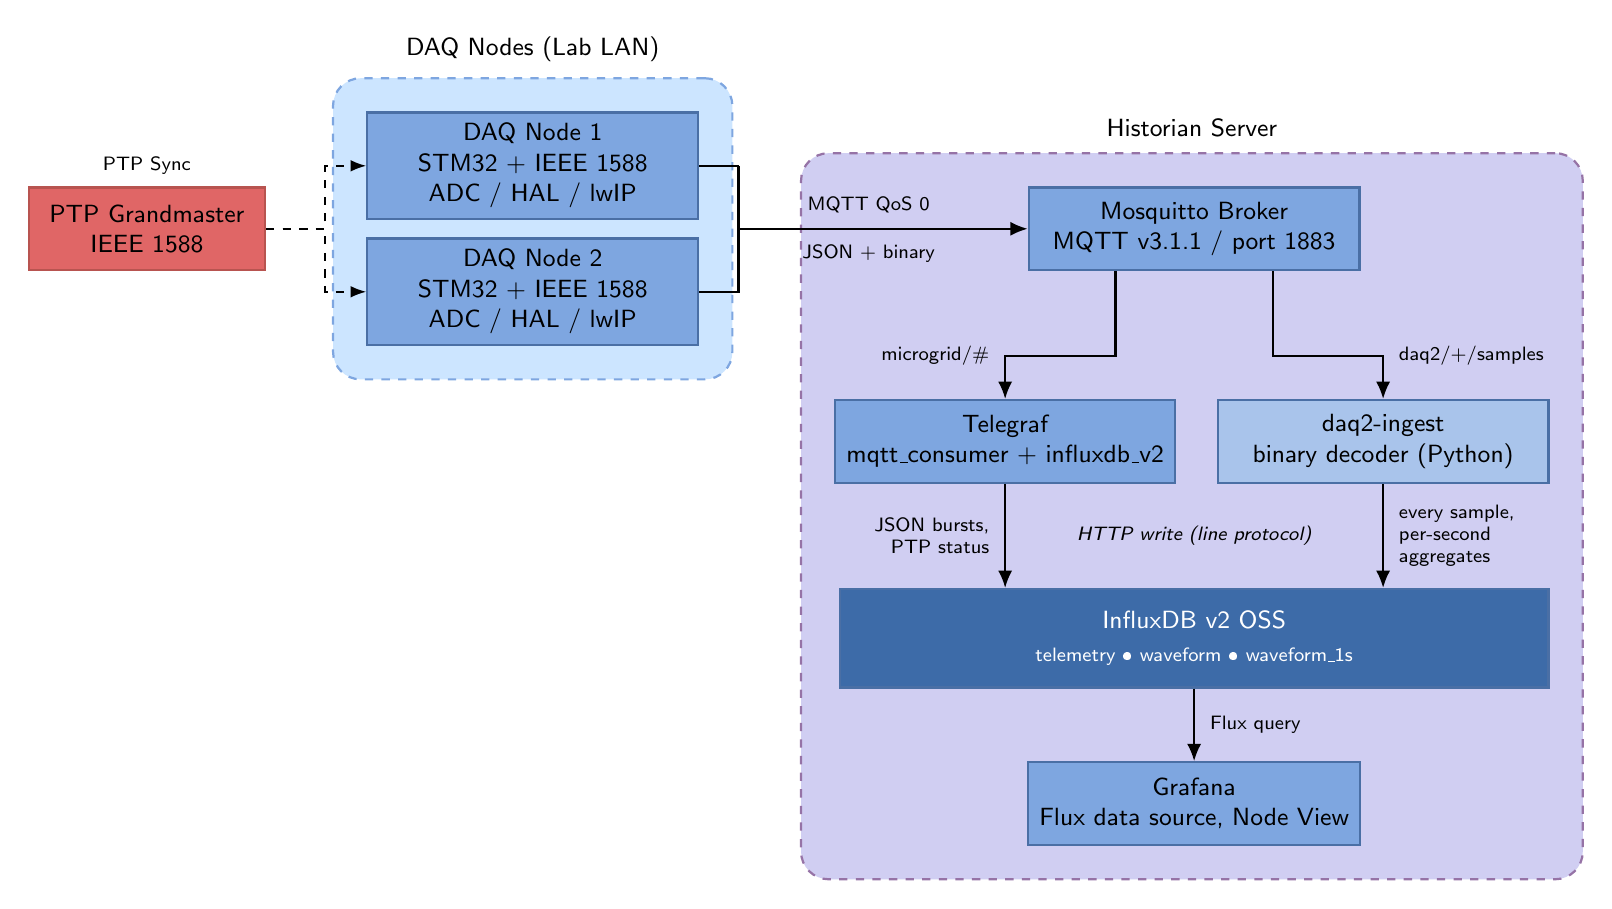
\begin{tikzpicture}
  % DAQ nodes
  \node[box] (n1) at (0, 0.8) {DAQ Node 1\\STM32 + IEEE 1588\\ADC / HAL / lwIP};
  \node[box] (n2) at (0, -0.8) {DAQ Node 2\\STM32 + IEEE 1588\\ADC / HAL / lwIP};
  \node[gm] (gm) at (-4.9, 0) {PTP Grandmaster\\IEEE 1588};

  % Historian server
  \node[box] (mq) at (8.4, 0) {Mosquitto Broker\\MQTT v3.1.1 / port 1883};
  \node[box] (tg) at (6.0, -2.7) {Telegraf\\mqtt\_consumer + influxdb\_v2};
  \node[box, fill=newfill] (dq) at (10.8, -2.7) {daq2-ingest\\binary decoder (Python)};
  \node[db, minimum width=9.0cm, minimum height=1.25cm] (ix) at (8.4, -5.2)
    {InfluxDB v2 OSS\\[1pt]\scriptsize telemetry \textbullet\ waveform \textbullet\ waveform\_1s};
  \node[box] (gf) at (8.4, -7.3) {Grafana\\Flux data source, Node View};

  \begin{scope}[on background layer]
    \node[group, draw=daqline, fill=daqgroup, fit=(n1)(n2)] (daqg) {};
    \node[group, draw=srvline, fill=srvgroup, fit=(mq)(tg)(dq)(ix)(gf)] (srvg) {};
  \end{scope}
  \node[glabel, above=2pt of daqg.north] {DAQ Nodes (Lab LAN)};
  \node[glabel, above=2pt of srvg.north] {Historian Server};

  % PTP
  \draw[sync] (gm.east) -- ++(0.75,0) |- (n1.west);
  \draw[sync] (gm.east) -- ++(0.75,0) |- (n2.west);
  \node[lbl, above=1pt of gm.north] {PTP Sync};

  % Nodes to broker
  \coordinate (join) at ($(n1.east) + (0.5,0)$);
  \draw[line width=0.8pt] (n1.east) -| (join);
  \draw[line width=0.8pt] (n2.east) -| (join);
  \draw[flow] (join |- mq.west) -- (mq.west)
    node[lbl, pos=0.45, above=2pt] {MQTT QoS 0}
    node[lbl, pos=0.45, below=2pt] {JSON + binary};

  % Broker to subscribers
  \draw[flow] (mq.south) ++(-1.0,0) |- ($(tg.north)+(0,0.55)$) -- (tg.north)
    node[lbl, pos=0.0, left=2pt] {microgrid/\#};
  \draw[flow] (mq.south) ++(1.0,0) |- ($(dq.north)+(0,0.55)$) -- (dq.north)
    node[lbl, pos=0.0, right=2pt] {daq2/+/samples};

  % Subscribers to InfluxDB
  \draw[flow] (tg.south) -- (tg.south |- ix.north)
    node[lbl, midway, left=2pt, align=right] {JSON bursts,\\PTP status};
  \draw[flow] (dq.south) -- (dq.south |- ix.north)
    node[lbl, midway, right=2pt] {every sample,\\per-second\\aggregates};
  \node[lbl, font=\sffamily\scriptsize\itshape] at ($(tg.south)!0.5!(dq.south |- ix.north)$)
    {HTTP write (line protocol)};

  % InfluxDB to Grafana
  \draw[flow] (ix.south) -- (gf.north) node[lbl, midway, right=2pt] {Flux query};
\end{tikzpicture}
\end{document}
